\documentclass[11pt]{article}
\usepackage[margin=2.6cm]{geometry}
\usepackage{amsmath,amssymb,amsthm}
\usepackage{tikz}
\usetikzlibrary{arrows.meta,positioning,decorations.pathmorphing}
\usepackage{booktabs}
\usepackage[colorlinks=true,linkcolor=blue!60!black,citecolor=blue!60!black]{hyperref}
\usepackage{tcolorbox}

\newtheorem{theorem}{Theorem}
\newtheorem{lemma}{Lemma}
\newtheorem{remark}{Remark}
\newtcolorbox{toolbox}[1]{colback=blue!4,colframe=blue!40!black,title={#1},fonttitle=\bfseries}
\newtcolorbox{examplebox}[1]{colback=green!4,colframe=green!35!black,title={#1},fonttitle=\bfseries}

\newcommand{\X}{X_{1,1}}
\newcommand{\CP}{\mathbb{CP}}
\newcommand{\R}{\mathbb{R}}
\newcommand{\Z}{\mathbb{Z}}
\newcommand{\tr}{\operatorname{tr}}
\newcommand{\Iw}{I_w}
\newcommand{\hb}{\hbar}

\title{\textbf{Which $SU(3)$? A didactic tour of Kaluza--Klein model building\\ on the Aloff--Wallach space $\X$}\\[1ex]
\large Charges, slots, and obstructions --- recovering the 1980s technology}
\author{kkFable working notes\thanks{Compiled from the derivation notes N0--N12 of the kkFable workspace
(2026-06-11/12); every load-bearing claim is re-derived by hand there, with two independent
verification passes recorded. This document is pedagogical: it narrates, the notes prove.}}
\date{June 12, 2026}

\begin{document}
\maketitle

\begin{abstract}
\noindent In the early 1980s it was briefly reasonable to hope that the Standard Model was
pure geometry: gauge bosons from isometries of a small seven-dimensional space, charges from
its bundles, couplings from its shape. The hope died for specific, instructive reasons that
are no longer taught. We revisit that technology on one concrete carrier --- the Aloff--Wallach
space $\X=SU(3)/U(1)_{1,1}$, an $SO(3)$ bundle over $\CP^2$ --- and work one sharp question
end to end: \emph{which $SU(3)$ does the base carry, the electroweak one (Option A) or QCD
colour (Option B)?} The answer is a tour of everything a young model builder needs from the
old toolbox: the isometry$\to$gauge-boson rule, Weinberg's coupling-from-inertia formula,
coset harmonics and equivariant bundles, spin$^c$ structures and charge parity, index-theorem
generation counting --- each with the explicit Lagrangian it descends from. Option B turns out
to reproduce the Standard Model's charge lattice with surgical near-misses: five of seven
matter slots land exactly, the electron singlet hides in the gravitino sector at the
canonical-bundle twist, the Higgs is forced out of scalar harmonics into internal tensor
components, and two obstructions remain irreducible --- there is no room for a dynamical
hypercharge boson, and no chirality. Chasing those two through the dimensional ladder
$D5\!-\!D6\!-\!D7$ (total spacetime $9/10/11$) reveals an electroweak alternation, a
charge-to-flux conversion law, and a transition whose endpoint realizes, at once, the two
ways a gauge sector can leave a theory: the vacuum running to infinity, or the coupling.
We keep $c=1$ but write $\hb$ and $\kappa^2=8\pi G$ explicitly throughout, so the reader can
see which statements are classical geometry and which are quantum spectroscopy.
\end{abstract}

\tableofcontents

%======================================================================
\section{Introduction: a lost subject}
%======================================================================

Between roughly 1979 and 1985 a substantial part of the high-energy community tried to derive
the Standard Model from pure gravity in eleven dimensions. The programme had crisp early
victories. Witten observed that seven is the \emph{minimal} number of extra dimensions whose
isometries can contain $SU(3)\times SU(2)\times U(1)$, and that eleven is also the maximal
dimension for supergravity --- a coincidence that still deserves a moment of silence
\cite{Witten81}. The seven-manifolds that realize the full Standard Model gauge group were
classified (the $M^{pqr}$ spaces, circle bundles over $\CP^2\times S^2$
\cite{Witten81,CDF84,FabbriFre99}); Weinberg showed that gauge couplings are computable
moments of inertia of the internal shape \cite{Weinberg83}; and the machinery of coset
harmonics turned spectroscopy into representation theory \cite{SalamStrathdee,DNP86}.

Then came the three deaths, all instructive: no chirality (massless fermions on smooth
odd-dimensional internal spaces pair left with right \cite{Witten81,Witten83}); no usable
vacuum (the natural ground states are anti-de Sitter at the compactification scale); and no
Standard-Model matter in the harmonic towers (the $M^{pqr}$ spectra simply do not contain the
quark and lepton representations \cite{FabbriFre99}). The community moved on to strings, and
the specific \emph{techniques} --- how to read charges off a coset, where hypercharge actually
lives, why the Higgs refuses to be a scalar harmonic --- quietly left the curriculum.

This paper is a guided tour of those techniques on a single, particularly instructive
carrier, with a single organizing question. The carrier is the Aloff--Wallach space
\begin{equation}
\X \;=\; SU(3)/U(1)_{1,1},\qquad U(1)_{1,1}=\{\,\mathrm{diag}(z,z,z^{-2})\,\},
\end{equation}
a seven-dimensional homogeneous space fibred as $SO(3)\to \X\to \CP^2$. It is, in a precise
sense, the \emph{other} natural seven-manifold built from $SU(3)$: where the $M^{pqr}$ spaces
keep a hypercharge circle and pay for it elsewhere, $\X$ trades that circle away for a fibre
with the shape of the weak group. The question is the fork that names this paper:
\begin{center}
\emph{The base $\CP^2=SU(3)/U(2)$ has isometry $SU(3)$ and isotropy $U(2)$.\\
Is that $SU(3)$ the electroweak $SU(3)$ of a 3-3-1 model (Option A),\\
or is it QCD colour, with the fibre $SO(3)$ as the weak group (Option B)?}
\end{center}
Option A was the assumption of all earlier work on this geometry; Option B is the flip.
Resolving the flip turns out to exercise every tool in the 1980s box exactly once, and the
near-misses are more instructive than the failures. Everything below is elementary --- the
point is precisely that it is elementary and yet nobody under fifty seems to know it.

\paragraph{Units.} We set $c=1$ and keep $\hb$ and the gravitational coupling
$\kappa^2 = 8\pi G$ \emph{visible}. The payoff is didactic: formulas containing only
$\kappa$ are classical geometry (couplings, masses of gauge bosons from shapes); $\hb$ enters
exactly where momentum is quantized on a compact direction (Kaluza--Klein masses, charge
quantization) and in loop quantities like $\alpha_a = \hb g_a^2/4\pi$. Watching where $\hb$
does \emph{not} appear is half the lesson.

%======================================================================
\section{The toolbox: Kaluza--Klein in five moves}
%======================================================================

\subsection{Move 1: isometries become gauge bosons}

Take $(4+d)$-dimensional gravity on $M_4\times X_d$,
\begin{equation}
S \;=\; \frac{1}{2\hat\kappa^2}\int d^{4+d}x\,\sqrt{-\hat g}\;\hat R ,
\qquad \hat\kappa^2 = 8\pi \hat G .
\label{eq:parent}
\end{equation}
If $X_d$ has isometry group $G_{\rm iso}$ with Killing vectors $K_a$, the metric fluctuation
\begin{equation}
ds^2 \;=\; g_{\mu\nu}(x)\,dx^\mu dx^\nu \;+\; g_{mn}(y)\,
\big(dy^m + K^m_a(y) A^a_\mu(x)\,dx^\mu\big)\big(dy^n + K^n_b(y) A^b_\nu(x)\,dx^\nu\big)
\label{eq:ansatz}
\end{equation}
is consistent at the massless level, and inserting it into \eqref{eq:parent} produces
four-dimensional Einstein--Yang--Mills theory: \emph{one massless gauge boson per Killing
vector, gauge group $=$ the isometry group}. No further choice is available: you cannot order
more gauge symmetry than the shape possesses. This single sentence already decides a large
part of our fork (Section~\ref{sec:rank}).

\begin{examplebox}{Example 1: the original circle, with $\hb$ and $\kappa$ in their places}
$X=S^1$ of circumference $L$, coordinate $y\in[0,L)$, one Killing vector $\partial_y$:
\[
ds^2 = g_{\mu\nu}dx^\mu dx^\nu + \rho^2\big(dy + A_\mu dx^\mu\big)^2 .
\]
Insert into \eqref{eq:parent} with $d=1$ and integrate over $y$:
\[
S_4=\int d^4x \sqrt{-g}\;\Big[\frac{\rho L}{2\hat\kappa^2}\,R
\;-\;\frac{\rho^3 L}{8\hat\kappa^2}\,F_{\mu\nu}F^{\mu\nu}
\;+\;\frac{L}{2\hat\kappa^2}\,(\text{gradient terms for }\rho)\Big].
\]
Reading off: $\;\kappa^2 \equiv \hat\kappa^2/(\rho L)$ \;and\;
$\dfrac{1}{g^2} = \dfrac{\rho^3 L}{2\hat\kappa^2}$ ---
\emph{both classical: no $\hb$ anywhere.} Quantum mechanics enters through the modes
$\phi_n \propto e^{2\pi i n y/L}$: their 4D masses and charges are
\[
m_n \;=\; \frac{2\pi \hb\,|n|}{\rho L}, \qquad
q_n \;=\; n \quad(\text{in units of } g),
\]
i.e.\ $\hb$ appears exactly once, multiplying the quantized circle momentum. Charge
quantization is momentum quantization --- Klein's 1926 observation, still the cleanest
sentence in the subject.
\end{examplebox}

\subsection{Move 2: couplings are moments of inertia (Weinberg's rule)}

For a general $X_d$ the same reduction gives, per isometry direction $a$,
\begin{equation}
\boxed{\;\frac{1}{g_a^2} \;=\; \frac{1}{2\hat\kappa^2}\int_{X_d}\!\sqrt{g_X}\;
g_{mn}\,K^m_a K^n_a \;\equiv\; \frac{I_a}{2\hat\kappa^2}\;}
\label{eq:inertia}
\end{equation}
--- the \emph{moment of inertia} of the internal shape about the axis $a$
\cite{Weinberg83}. Two consequences organize everything later:
\begin{itemize}
\item If two generators sit inside one \emph{simple} isometry factor, Schur's lemma forces
their inertias into a fixed ratio: the corresponding coupling ratio is \emph{group theory},
not geometry. (This is how Option A predicts $\sin^2\theta_W = 1/4$.)
\item If they sit in \emph{different} factors of a semisimple isometry group, the ratio is a
free shape modulus. (This is how Option B loses that prediction.)
\end{itemize}

\subsection{Move 3: spectroscopy is representation theory (Frobenius)}

\begin{toolbox}{The one formula to remember}
Fields on $X=G/H$ valued in the homogeneous bundle of the $H$-module $W$, twisted by a
background flux line $\mathcal O(m)$, have 4D mode content
\[
\text{modes} \;=\; \bigoplus_{\lambda}\; V_\lambda \;\otimes\;
\mathrm{Hom}_H\!\big(V_\lambda,\; W\otimes \mathcal O(m)\big),
\]
i.e.\ a mode in the $G$-irrep $V_\lambda$ exists iff $V_\lambda$, restricted to $H$, contains
the $H$-type of the bundle. \emph{All} charge bookkeeping below is this one line, evaluated
on small tables. For $\X$, $H=U(1)_{1,1}$ is tiny, so the condition is a single charge
balance: $q_8(\text{state}) + q_8(W\text{-component}) + m = 0$, where $q_8$ is the eigenvalue
of $\mathrm{diag}(1,1,-2)$.
\end{toolbox}

\subsection{Move 4: fermions see double covers (and a one-line parity law)}

Spinor fields transform under the \emph{double cover} of the isometry/isotropy groups: they
may carry half-integer labels that bosons cannot. On $\X$ this is governed by one group
element, which deserves a box because it will do a remarkable amount of work:

\begin{toolbox}{The parity element $\zeta$}
Let $\zeta=\exp\big(i\pi\,\mathrm{diag}(1,1,-2)\big)=\mathrm{diag}(-1,-1,1)\in SU(3)$.
This single element lies \emph{both} in the quotient circle $U(1)_{1,1}$ (at $z=-1$)
\emph{and} in the upper-block $SU(2)$ (as its centre $-\mathbf 1_2$). Evaluate it twice on
any weight state of any $SU(3)$ representation:
\[
(-1)^{q_8} \;=\; \zeta \;=\; (-1)^{2I}
\qquad\Longrightarrow\qquad
\boxed{\,q_8 \equiv 2I \pmod 2\,}.
\]
Doublet-ness and charge parity are locked: every $SU(2)$ doublet carries odd $q_8$, every
singlet/triplet even $q_8$. Geometrically this $\mathbb Z_2$ is simultaneously (i) the
obstruction to lifting the fibre $SO(3)$ to $SU(2)$, (ii) the non-spin-ness of $\CP^2$
repaired by odd flux (the spin$^c$ condition), and (iii) --- as we will see --- the seed of the
Standard Model's $\mathbb Z_6$ charge correlation.
\end{toolbox}

\subsection{Move 5: the chirality wall}

On a smooth, compact, \emph{odd}-dimensional internal space the internal Dirac operator has
no chirality grading; its modes pair into 4D left--right couples with identical quantum
numbers. The spectrum is vector-like, no matter how clever the bundles
\cite{Witten81,Witten83}. Twisting by spin$^c$ lines does not evade it. Every slot statement
in this paper is therefore a statement about \emph{vector-like pairs}; producing a chiral
spectrum needs an even-dimensional stage (Section~\ref{sec:ladder}) or singular geometry
\cite{KK2025}. Keeping this wall visible at all times was a 1980s discipline worth reviving.

%======================================================================
\section{The carrier: $\X$ in one section}
%======================================================================

\begin{figure}[t]
\centering
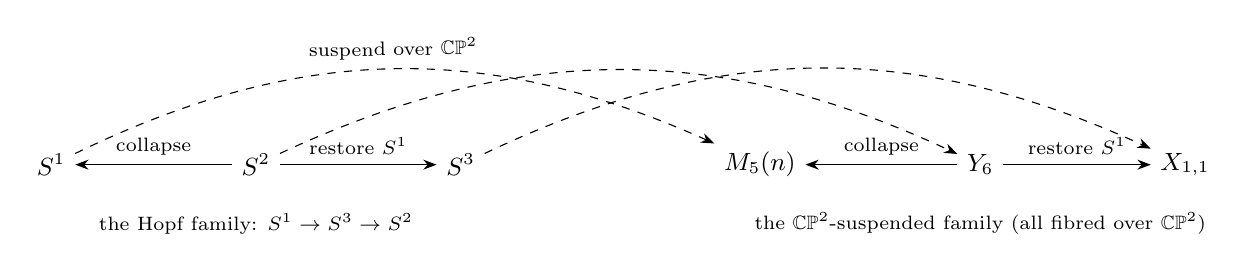
\begin{tikzpicture}[>=Stealth, every node/.style={font=\small}]
% Low-dimensional Hopf ladder
\node (S1) at (0,0) {$S^1$};
\node (S2) at (2.6,0) {$S^2$};
\node (S3) at (5.2,0) {$S^3$};
\draw[<-] (S1) -- node[above]{\scriptsize collapse} (S2);
\draw[->] (S2) -- node[above]{\scriptsize restore $S^1$} (S3);
\node at (2.6,-0.75) {\scriptsize the Hopf family: $S^1\to S^3\to S^2$};
% suspended ladder
\node (M5) at (9.0,0) {$M_5(n)$};
\node (Y6) at (11.8,0) {$Y_6$};
\node (X7) at (14.4,0) {$\X$};
\draw[<-] (M5) -- node[above]{\scriptsize collapse} (Y6);
\draw[->] (Y6) -- node[above]{\scriptsize restore $S^1$} (X7);
\node at (11.8,-0.75) {\scriptsize the $\CP^2$-suspended family (all fibred over $\CP^2$)};
% vertical arrows
\draw[->,dashed] (S1) to[bend left=25] node[above,sloped]{\scriptsize suspend over $\CP^2$} (M5);
\draw[->,dashed] (S2) to[bend left=25] (Y6);
\draw[->,dashed] (S3) to[bend left=25] (X7);
\end{tikzpicture}
\caption{The dimensional ladder. Left: the familiar Hopf triple. Right: its suspension over
$\CP^2$: the lens-space circle bundle $M_5(n)=S(\mathcal O(n))\simeq S^5/\Z_n$ (internal
$D5$, total spacetime $9$), the flag manifold $Y_6=SU(3)/T^2$ (an $S^2$ bundle over $\CP^2$;
internal $D6$, total $10$), and the Aloff--Wallach space $\X$ (internal $D7$, total $11$).}
\label{fig:ladder}
\end{figure}

Three descriptions of one space, each carrying one physics lesson:

\textbf{(a) As a circle quotient.} $\X=SU(3)/U(1)_{1,1}$. The quotient circle is generated by
$H_8=\mathrm{diag}(1,1,-2)$ --- the \emph{hypercharge-shaped} direction of $SU(3)$ (it is the
centre of the block subgroup $U(2)=S(U(2)\times U(1))$). Lesson: the circle you divide out
acts trivially on the quotient; \emph{whatever physics you wanted from it can only survive
as bundle data, never as a gauge boson}.

\textbf{(b) As a bundle.} The right action of $U(2)/U(1)_{1,1}=PU(2)\cong SO(3)$ survives the
quotient and rotates the fibres of $SO(3)\to \X\to \CP^2$: a fibre shaped like the
(adjoint of the) weak group over a base shaped like a colour space. The full isometry group
is $SU(3)\times SO(3)$ (Wilking), of rank $2+1=3$. The tangent space splits into the fibre
block $m_0$ (3 directions, $q_8=0$, metric scale $x_1$) and the base block $m_3$
(4 directions, $q_8=\pm3$, scale $x_2$); the shape modulus $t = x_1/x_2-1$ has two Einstein
points, $t=+1$ (3-Sasakian) and $t=-3/5$ (squashed) --- remember those two wells, they return
in Section~\ref{sec:ladder}.

\textbf{(c) As a rung.} Inside the maximal torus $T^2\subset SU(3)$ live two orthogonal
circles: the $Y$-circle ($H_8$) and the $T_3$-circle ($H_3=\mathrm{diag}(1,-1,0)$). The three
spaces of Figure~\ref{fig:ladder} are the three ways of distributing them between geometry
and flux:
\begin{center}
\begin{tabular}{lccc}
\toprule
rung & gauged (isometry) & flux (bundle label) & rank \\
\midrule
$D5$: $M_5(n)$ & $SU(3)\times U(1)_Y$ & weak data absent & 3\\
$D6$: $Y_6$ & $SU(3)$ only & both: base flux $n$, monopole $r$ & 2\\
$D7$: $\X$ & $SU(3)\times SO(3)_{\rm weak}$ & hypercharge flux $n$ & 3\\
\bottomrule
\end{tabular}
\end{center}
\emph{On no rung are both electroweak circles geometric} --- the alternation that drives
Section~\ref{sec:ladder}. The Standard Model needs rank 4 on one space; this family caps at 3.

%======================================================================
\section{The fork, part I: gauge bosons and the rank budget}\label{sec:rank}
%======================================================================

Under Option A the electroweak pair $(T_3, Y)$ sits inside the simple base $SU(3)$: rank 2 of
the available 3, with the fibre $SO(3)$ left over as a custodial spectator. The budget
closes, at the price of having no colour anywhere.

Under Option B, colour consumes the whole $SU(3)$ (both Cartans are gluons --- and note that
no hypercharge can hide inside colour: $Z(\mathfrak{su}(3))=0$), the weak group consumes the
fibre Cartan, and the count reads
\[
\underbrace{2}_{\text{gluons}}+\underbrace{1}_{W^3}+\underbrace{1}_{B}\;=\;4
\;>\;3\;=\;\mathrm{rank}\big(SU(3)\times SO(3)\big).
\]
One boson is missing, and it is precisely hypercharge. The would-be $Y$ circle is the
quotient circle of description (a): trivial action, no Killing vector, no gauge field. The
candidate repairs all die by short arguments: the bare double cover $SO(3)\to SU(2)$ adds no
Cartan; a Betti $U(1)$ from the 3-form on the harmonic 2-form ($b_2(\X)=1$) exists in
supergravity embeddings but \emph{every Kaluza--Klein state is neutral under it} --- a fact
the $M^{111}$ harmonic analysis states verbatim \cite{FabbriFre99}.

\begin{examplebox}{Example 2: the Lagrangian that is missing a term}
Reducing \eqref{eq:parent} on $(\X, g_t)$ with the rule \eqref{eq:inertia} gives, under
Option B,
\[
\mathcal L_4 \;=\; \frac{1}{2\kappa^2}R
\;-\;\frac{x_2 V_7}{8\hat\kappa^2}\,\tr G_{\mu\nu}G^{\mu\nu}
\;-\;\frac{x_1 V_7}{8\hat\kappa^2}\,\tr W_{\mu\nu}W^{\mu\nu}
\;-\;\frac{M_P^2}{2}(\partial\sigma)^2\;+\;\dots
\]
($G$: gluons; $W$: the fibre $SO(3)$; $\sigma$: moduli). The term
$-\frac14 g_Y^{-2}B_{\mu\nu}B^{\mu\nu}$ \emph{does not exist}: there is no eleventh Killing
vector to generate it. Every formula of electroweak phenomenology that divides by $g'$
divides by zero on this carrier. Note also what the two visible coefficients say:
$g_2^2/g_3^2 = x_2/x_1$ is a free shape ratio (two factors, no Schur lock), so even
colour--weak unification statements are moduli, not predictions.
\end{examplebox}

The same calculus kills the angle. Counterfactually granting a $Y$ boson normalized on the
base block with strength $k_Y$,
\begin{equation}
\sin^2\theta_W \;=\; \frac{g_Y^2}{g_2^2+g_Y^2}\;=\;\frac{x_1}{x_1+k_Y x_2}
\;=\;\frac{1+t}{(1+t)+k_Y}\,,
\end{equation}
monotone in the free modulus $t$: every value in $(0,1)$ is attained. Contrast Option A,
where both generators live in one simple factor and Schur fixes
$\sin^2\theta_W=\tr T_3^2/\tr Q^2 = 1/4$ on the lepton triplet, metric-independently. This is
the cleanest classroom example we know of Weinberg's dichotomy: \emph{same geometry, same
formula \eqref{eq:inertia}, and the answer flips from ``rigid number'' to ``free dial''
purely according to where the generators sit.}

%======================================================================
\section{The fork, part II: the charge lattice and the matter slots}
%======================================================================

Now the spectroscopy. Apply the Frobenius box with the branching data of $SU(3)$
($\mathbf 3 = \mathbf 2_{+1}\oplus\mathbf 1_{-2}$ under $SU(2)\times U(1)_8$, etc.), the
spinor module
\[
\Delta_7 \;=\; \mathbf 2_{+3}\oplus\mathbf 2_{-3}\oplus\mathbf 3_0\oplus\mathbf 1_0 ,
\]
and the normalization $Y=m/6$ for the flux charge $m$ (forced, not chosen: see below).
Under Option B the 4D colour representation is the $SU(3)$ label $\lambda$, the weak isospin
$\Iw$ is the combined $SU(2)$ spin, and one finds (notes N6):

\begin{center}
\begin{tabular}{lccl}
\toprule
SM slot & $(\text{colour},\Iw,Y)$ & twist $m$ & status on $\X$ (Dirac sector)\\
\midrule
$Q_L$ & $(\mathbf 3,\tfrac12,+\tfrac16)$ & $\mp1$ & exists\\
$u_R$ & $(\mathbf 3,0,+\tfrac23)$ & $\mp4$ & exists\\
$d_R$ & $(\mathbf 3,0,-\tfrac13)$ & $\pm2$ & exists\\
$L$ & $(\mathbf 1,\tfrac12,-\tfrac12)$ & $\pm3$ & exists \emph{(fixes the unit $Y=m/6$)}\\
$\nu_R$ & $(\mathbf 1,0,0)$ & $0$ & exists\\
$e_R$ & $(\mathbf 1,0,-1)$ & $\pm6$ & \textbf{absent} (selection rule)\\
$H$ & $(\mathbf 1,\tfrac12,+\tfrac12)$, scalar & --- & \textbf{absent} (scalar fields)\\
\bottomrule
\end{tabular}
\end{center}

Five slots land on exact Standard-Model hypercharges with a single normalization constant;
the geometry even enforces the Standard Model's global $\mathbb Z_6$ structure,
\begin{equation}
6Y \;\equiv\; 2\,t(\lambda) + 3\,(2\Iw) \pmod 6
\end{equation}
($t=$ triality) --- the $\zeta$-parity law and the triality lock combined, which is precisely
the charge correlation that makes the SM gauge group $[SU(3)\times SU(2)\times U(1)]/\Z_6$.
And then two slots fail, by clean selection rules: a colour-singlet weak-singlet fermion is
pinned to $Y=0$ (so no $e_R$), and a colour-singlet weak-doublet \emph{scalar field} does not
exist for any twist (so no elementary Higgs). Selective failure of exactly two occupants of
an otherwise perfect lattice is the signature of structure, not accident --- and indeed both
absences have mechanisms, and both mechanisms have escapes.

\subsection{The electron hides in the gravitino (charge doubling)}

The Dirac-sector bound is $|q_8(\Delta_7)|\le 3$, and worse, $\Iw=0$ forces the neutral
component. But eleven-dimensional supergravity offers one more fermionic bundle: the
\emph{internal gravitino components} $\psi_m$, which are 4D spin-$\tfrac12$ fields valued in
$W=\Delta_7\otimes m$. Decomposing (notes N11, independently verified):
\[
\Delta_7\otimes m \;\supset\; \mathbf 1_{+6}\oplus \mathbf 1_{-6}
\quad\text{(exactly one each),}
\]
because the spinor and tangent bundles of $\X$ \emph{share the same charged doublet}
$\mathbf 2_{\pm3}$, and $\mathbf 2\otimes\mathbf 2\to\mathbf 1$ \emph{adds the charges}:
$3+3=6$. The resulting slot is $(\mathbf 1, 0, Y=\mp1)$ at twist $m=\pm6$: the right-handed
electron, at \emph{twice the lepton-doublet twist} --- in the same unit $Y=m/6$ fixed by $L$,
with no new freedom. Three remarks make this more than a curiosity:
\begin{enumerate}
\item \emph{It is the canonical-bundle locus.} On $\CP^2$ alone, Dolan and Nash found $e_R$
at the twist $q=-3$, the canonical bundle $K$ \cite{DolanNash02}; the $\X$ slot at $|m|=6$ is
its 7D avatar ($\Lambda^2\mathbf 2_{+3}=\mathbf 1_{+6}$). The electron singlet persistently
sits where the spin$^c$ geometry is most twisted.
\item \emph{The mechanism is rigid.} Doubling needs the tangent and spinor bundles to share
one odd-charged doublet. On $S^5\times S^2$ the tangent charge is too small and the doubled
charges come out as doublets, not singlets: no $e_R$ there, verifiably. On $M^{111}$ the
\emph{only} massless charged colour/weak singlets in the entire computed spectrum are the two
gravitini \cite{FabbriFre99}. Across every carrier examined: \emph{if this family has an
electron, it is gravitino-borne.}
\item \emph{It survives gauge fixing.} The $\gamma$-trace and longitudinal pieces of
$\psi_m$ remove one $\Delta_7$'s worth of states, all bounded by $|q_8|\le3$: the $\pm6$
singlets are untouchable.
\end{enumerate}

\subsection{The Higgs is forced into the internal geometry}

The scalar no-go has the same texture. A 4D scalar descending from a scalar \emph{field} on
$\X$ sits in $W=\mathbf 1$: colour-singlet $\Rightarrow$ charge balance at $q_8=0$
$\Rightarrow$ integer $\Iw$. No doublet, ever. But scalars also descend from \emph{internal
tensor components} --- and there the doublets reappear:
\[
\Lambda^3 m \;\supset\; 2\cdot \mathbf 2_{\pm3}\oplus\mathbf 4_{\pm3}, \qquad
\mathrm{Sym}^2 m \;\supset\; \mathbf 2_{\pm3}\oplus\mathbf 4_{\pm3},
\]
so the 3-form components $A_{mnp}$ and the mixed metric components $g_{(fibre,base)}$, at
twist $|m|=3$, furnish colour-singlet $\Iw=\tfrac12$ scalars at $Y=\pm\tfrac12$: Higgs
quantum numbers. The lesson generalizes into a slogan the 1980s learned the hard way and we
can now state as a selection rule: \emph{the Standard-Model Higgs cannot be a scalar
harmonic; if geometry provides it at all, it provides it as an internal component of a
higher-spin field} --- which is exactly the ansatz of coset-space dimensional reduction and
of modern gauge--Higgs unification. What looked like a modelling preference is a theorem
about charge locking.

\begin{figure}[t]
\centering
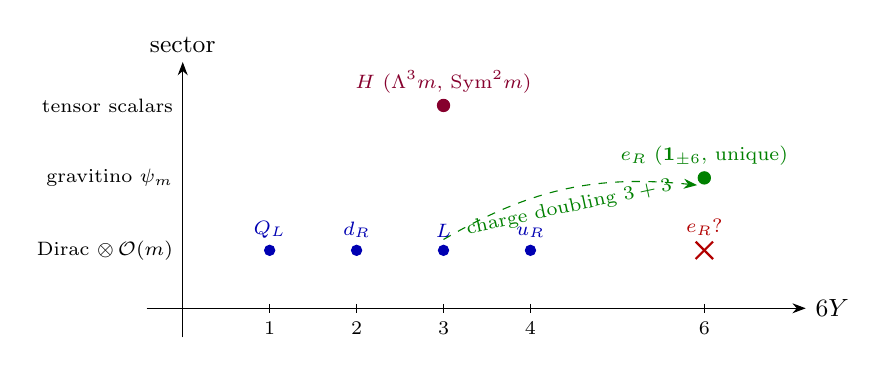
\begin{tikzpicture}[>=Stealth,scale=0.92, every node/.style={font=\small}]
% axes
\draw[->] (-0.5,0) -- (8.6,0) node[right]{$6Y$};
\draw[->] (0,-0.4) -- (0,3.4) node[above]{sector};
\foreach \x in {1,2,3,4,6} \draw (\x*1.2,0.06) -- (\x*1.2,-0.06) node[below]{\scriptsize \x};
% rows
\node[left] at (0,0.8) {\scriptsize Dirac $\otimes\,\mathcal O(m)$};
\node[left] at (0,1.8) {\scriptsize gravitino $\psi_m$};
\node[left] at (0,2.8) {\scriptsize tensor scalars};
% Dirac slots
\filldraw[blue!70!black] (1.2*1,0.8) circle (2pt) node[above=1pt]{\scriptsize $Q_L$};
\filldraw[blue!70!black] (1.2*2,0.8) circle (2pt) node[above=1pt]{\scriptsize $d_R$};
\filldraw[blue!70!black] (1.2*3,0.8) circle (2pt) node[above=1pt]{\scriptsize $L$};
\filldraw[blue!70!black] (1.2*4,0.8) circle (2pt) node[above=1pt]{\scriptsize $u_R$};
\draw[red!70!black, thick] (1.2*6+0.12,0.68) -- (1.2*6-0.12,0.92);
\draw[red!70!black, thick] (1.2*6-0.12,0.68) -- (1.2*6+0.12,0.92);
\node[red!70!black] at (1.2*6,1.12) {\scriptsize $e_R$?};
% gravitino slots
\filldraw[green!50!black] (1.2*6,1.8) circle (2.4pt) node[above=1pt]{\scriptsize $e_R$ ($\mathbf 1_{\pm6}$, unique)};
\draw[->,green!50!black,dashed] (1.2*3,0.95) to[bend left=18] node[below,sloped]{\scriptsize charge doubling $3+3$} (1.2*6-0.1,1.7);
% tensor scalars
\filldraw[purple!70!black] (1.2*3,2.8) circle (2.4pt) node[above=1pt]{\scriptsize $H$ ($\Lambda^3 m$, $\mathrm{Sym}^2 m$)};
\node[right] at (8.8,1.8) {};
\end{tikzpicture}
\caption{The colour-singlet charge ladder on $\X$ under Option B (charges in units
$6Y=m$). The Dirac sector reaches $|6Y|\le 3$ for singlets and places five SM slots; $e_R$
at $|6Y|=6$ is reachable only by the gravitino components (charge doubling through the
shared doublet $\mathbf 2_{\pm3}$), and the Higgs only by internal tensor scalars at
$|6Y|=3$.}
\label{fig:slots}
\end{figure}

\subsection{Scorecard and the two irreducible obstructions}

With the supergravity field menu --- and nothing exotic added --- \emph{all seven} SM slots
exist on $\X$ under Option B. What remains impossible is carrier-level, not slot-level:
\begin{enumerate}
\item \textbf{No dynamical hypercharge boson} (the rank budget of Section~\ref{sec:rank});
\item \textbf{No chirality} (Move 5: every slot above is a vector-like pair).
\end{enumerate}
For comparison, the rank-complete carriers fail in the mirrored way: $M^{111}$ gauges the
full $SU(3)\times SU(2)\times U(1)$ but its harmonic lattice contains \emph{no $SU(2)$
doublets at any level and no charged colour-singlet matter} \cite{FabbriFre99};
$S^5\times S^2$ gauges rank 4 but lands only $Q_L$ and $L$. We call this pattern
\emph{complementary exclusion}: within the whole $SU(3)$-based family, gauge-rank
completeness and the doublet/lepton matter mechanism never coexist. The literature's one
working SM spectrum from these spaces --- Dolan--Nash's --- evades the dichotomy by gauging
\emph{holonomy} instead of isometry and paying with non-dynamical gauge fields
\cite{DolanNash02,DolanNash02b}; under an isometry reading, their construction is exactly
Option-A-shaped. Colour on the $\CP^2$ isometry is, in a precise sense, the one thing this
geometry refuses to subsidize fully.

%======================================================================
\section{The ladder: transitions, the two exits, and criticality}\label{sec:ladder}
%======================================================================

The two irreducible obstructions live on \emph{different rungs} of Figure~\ref{fig:ladder}:
$D5$ has the hypercharge boson; $D6$ is even-dimensional and can carry a chiral index
(this is where the generation count $\nu_n=(n^2-1)/8$ lives --- Appendix~\ref{app:index});
$D7$ has the weak group and the matter slots. The Standard Model, on this family, is
\emph{phase-distributed}. That makes the transitions between rungs the central object, and
here the 1980s technology connects to thoroughly modern questions.

\subsection{The $D7\to D6$ collapse is a quintet Higgsing}

Inside the invariant metric family of $\X$, split the fibre block:
$x_\parallel$ on the $T_3$ axis, $x_\perp$ on the rest. The space of fibre metrics is
$\mathrm{Sym}^2(\mathbf 3)=\mathbf 1\oplus\mathbf 5$ of the weak $SO(3)$: the breathing mode
and a \emph{quintet}. The axis squash is the $I_3=0$ component of the quintet, so the
collapse family is, in 4D language, a vacuum line of a colour-singlet, $\Iw=2$, $Y=0$ scalar
$\Phi_5$ --- an order parameter that breaks $SU(2)_L\to U(1)_{T_3}$ geometrically:

\begin{examplebox}{Example 3: the Lagrangian of a collapsing dimension}
Along the family $g(x_\parallel,x_\perp,x_2)$ the reduction gives (schematically but with
every coefficient's origin visible; $V=\sqrt{x_\parallel x_\perp^2 x_2^4}\cdot v_0$)
\[
\mathcal L_4 = \frac{1}{2\kappa^2}R
\;-\;\frac{x_\parallel V}{4\hat\kappa^2} F^{(T_3)}_{\mu\nu}F^{(T_3)\mu\nu}
\;-\;\frac{x_\perp V}{4\hat\kappa^2}\big|F^{(W^\pm)}_{\mu\nu}\big|^2
\;-\;\frac{M_P^2}{2}\,(\partial\sigma)^2
\;-\;M_W^2(\sigma)\,W^+_\mu W^{-\mu}\;-\;V(\sigma)+\dots
\]
with $\sigma \propto M_P\log(x_\perp/x_\parallel)$ the canonical quintet modulus and
$M_W^2 \propto g_2^2\langle\Phi_5\rangle^2$. The $T_3$ boson stays \emph{exactly massless}
at every $x_\parallel>0$ (it is an isometry of the whole family); the $W^\pm$ are Higgsed by
an $I_w=2$ vev --- which is \emph{not} the Standard-Model mechanism and protects nothing; it
is the ladder's own, geometric, Higgsing.
\end{examplebox}

Now send $x_\parallel\to0$ (Gromov--Hausdorff collapse $\X\to Y_6$, curvature bounded) and
watch the gauge sector leave the theory. It leaves \emph{twice, in the two inequivalent ways
a gauge sector can leave}:
\begin{itemize}
\item \textbf{The vev exit.} For $W^\pm$: $g_W$ stays finite while
$\sigma\to\infty$ --- infinite distance in moduli space, $M_W\to\infty$. The broken pair
decouples because \emph{the vacuum runs to infinity}.
\item \textbf{The coupling exit.} For the surviving $U(1)_{T_3}$: massless the whole way,
but $1/g_{T_3}^2\propto x_\parallel V\to0$. The boson leaves at \emph{zero mass through
infinite coupling}.
\end{itemize}
One transition, both exits, assigned by representation: broken non-abelian directions exit
through the vacuum, the surviving abelian through the coupling. Meanwhile the \emph{quantum
numbers} cross the transition smoothly: collapsing the circle converts the gauged $T_3$
charge of every mode into the monopole flux label of the limit,
\begin{equation}
r \;=\; 2I_3 ,
\end{equation}
which is precisely the vertical twist of the $D6$ fermion construction. Charge lattices
transport; gauge dynamics does not. The open dynamical question of this whole programme is
now locatable in one sentence: \emph{what is the strong-coupling fate of the abelian factor
at the endpoint --- confinement, duality, or absorption into the flux sector?}

\begin{figure}[t]
\centering
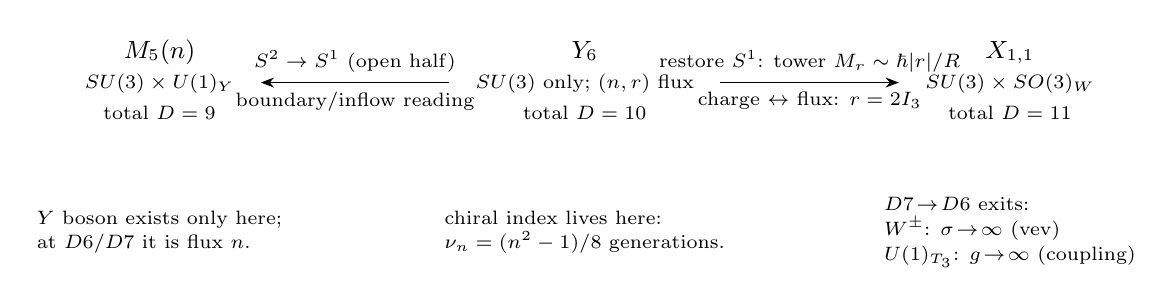
\begin{tikzpicture}[>=Stealth, every node/.style={font=\small}]
\node (D5) at (0,0) {\begin{tabular}{c}$M_5(n)$\\ \scriptsize $SU(3)\times U(1)_Y$\\ \scriptsize total $D=9$\end{tabular}};
\node (D6) at (5.4,0) {\begin{tabular}{c}$Y_6$\\ \scriptsize $SU(3)$ only; $(n,r)$ flux\\ \scriptsize total $D=10$\end{tabular}};
\node (D7) at (10.8,0) {\begin{tabular}{c}$\X$\\ \scriptsize $SU(3)\times SO(3)_W$\\ \scriptsize total $D=11$\end{tabular}};
\draw[<-] (D5) -- node[above]{\scriptsize $S^2\to S^1$ (open half)} node[below]{\scriptsize boundary/inflow reading} (D6);
\draw[->] (D6) -- node[above]{\scriptsize restore $S^1$: tower $M_r\sim \hb|r|/R$} node[below]{\scriptsize charge $\leftrightarrow$ flux: $r=2I_3$} (D7);
% exits annotation
\node[align=left] at (10.8,-1.9) {\scriptsize $D7\!\to\!D6$ exits:\\[-2pt] \scriptsize $W^\pm$: $\sigma\!\to\!\infty$ (vev)\\[-2pt] \scriptsize $U(1)_{T_3}$: $g\!\to\!\infty$ (coupling)};
\node[align=left] at (0,-1.9) {\scriptsize $Y$ boson exists only here;\\[-2pt] \scriptsize at $D6$/$D7$ it is flux $n$.};
\node[align=left] at (5.4,-1.9) {\scriptsize chiral index lives here:\\[-2pt] \scriptsize $\nu_n=(n^2-1)/8$ generations.};
\end{tikzpicture}
\caption{The electroweak alternation and the transitions. Restoration $D6\to D7$ passes the
M-theory-style tower test by construction (radius modulus, infinite flux family, gap closing
as $\hb|r|/R$); the collapse realizes the two exits; the $D6\leftrightarrow D5$ half remains
open, organized by the same vev-vs-coupling dichotomy.}
\label{fig:transitions}
\end{figure}

\subsection{Criticality: when is a jump a jump?}

A Higgs field breaks a symmetry only when its potential \emph{has the Mexican-hat shape}; a
parameter sliding continuously along a fixed potential changes nothing qualitative. The same
discipline applies to dimensions. Moving along the collapse family at $x_\parallel>0$ is
sliding a vev: nothing critical happens. The endpoint is different in kind: the dimension
drops, the isometry group jumps, and an \emph{infinite tower} of states
($M_r \sim \hb|r|/R$, $R\propto\sqrt{x_\parallel}$) degenerates at once. That tower is
exactly what distinguishes a genuine dimensional transition from a mere symmetry
restoration: Witten's IIA/M-theory jump supplied the benchmark (a radius growing with a
modulus, an infinite charge family, masses $\sim \hb|n|/R$) \cite{Witten95}, and the
restoration $D6\to D7$ satisfies all three ingredients \emph{literally}, because the circle
and its momentum tower are real geometry here. In total dimension this is a $10\to11$-type
jump: continuous control, critically discontinuous endpoint.

Where is the hat itself? The potential $V(\sigma)$ on the invariant moduli is not flat: on
the $t$-axis it has \emph{two} known stationary points --- the two Einstein metrics
($t=+1$ and $t=-3/5$) --- and the collapse direction is an infinite-distance runaway, not a
minimum. The sharp open problem, stated so a student could attack it: compute the reduced
potential $V(x_\parallel,x_\perp,x_2)$ (its $t$-axis restriction is already in the prior
literature of this programme), and determine which deformations --- flux $n$, curvature
couplings, a cosmological term --- move, merge, or create its wells. That is the
hat-formation analysis for a dimension, with the two Einstein points as its first data.

\subsection{Two views of one transition: collapse and emergence}

There is a question the reader should now ask, because Witten taught us all to ask it: we
\emph{derived} the transition downward ($D7\to D6$, a collapse), but the famous version runs
upward --- IIA string theory discovering its eleventh dimension as the coupling grows
\cite{Witten95}. Are both views suitable here? Yes --- and the asymmetry between them is the
last lesson of the tour.

\emph{The collapse view} takes the geometry as fundamental: the momentum tower
$M_r\sim\hb|r|/R$ decouples upward, the flux labels are the frozen memory of eaten charges.
Every step is a theorem of the metric family.

\emph{The emergence view} takes the $D6$ description as fundamental: one observes flux
sectors labelled by $r$, notices their spectrum organizing into a tower whose gap closes as
a modulus grows, and \emph{infers} a circle. This is exactly Witten's logic --- but his
version had a hidden ingredient. The IIA D0-brane tower is BPS: $M_n = |n|/(g_s\ell_s)$,
exactly linear in the charge, protected all the way to strong coupling. Here, near the $D6$
end, the lowest monopole-sector masses scale as $M_r\propto \hb\sqrt{|r|}/R_{S^2}$ (the
lowest monopole harmonic at $j=|r|/2$ has eigenvalue $j(j+1)-r^2/4 = |r|/2$): a
\emph{square-root} tower. Linearity in $|r|$ holds near the $D7$ end, in the momentum
regime; whether it survives deep collapse is precisely what supersymmetry guaranteed for
Witten and nothing guarantees in this bosonic family. So: \emph{collapse view --- a theorem;
emergence view --- Witten's reading minus the BPS protection}, with a well-posed open
problem in the gap: find, or exclude, a protection mechanism for the linear tower.

The gauge sector matches gratifyingly across the two readings. In IIA$\,\to\,$M the
Ramond--Ramond photon \emph{enters from strong coupling} as $R_{11}$ grows (the inertia rule
again: $1/g^2\propto R_{11}^3$); our $U(1)_{T_3}$ \emph{exits to strong coupling} under
collapse. Same phenomenon, opposite orientation --- and Witten's case is the existence proof
that the strong-coupling end of the coupling exit is physics, not pathology. Finally, the
criticality itself is frame-dependent in a precise sense: seen from $D7$ the endpoint is a
smooth infinite-distance limit; seen from $D6$ it is the nucleation of a new dimension ---
one transition, read from the ordered or the disordered side.

%======================================================================
\section{What the 1980s knew, in six lines}
%======================================================================

\begin{enumerate}
\item \textbf{You cannot gauge what you quotient.} The circle you divide out has no Killing
vector; its physics survives only as bundle data. (Where hypercharge went.)
\item \textbf{Couplings are inertias.} Ratios inside one simple factor are theorems; ratios
across factors are moduli. (Why $1/4$ was ever predicted, and why the flip unpredicts it.)
\item \textbf{Charges are weights, and fermions see double covers.} One central element can
lock parity ($q_8\equiv2I$), and through it, the SM's $\mathbb Z_6$. (Why the charge lattice
came out right.)
\item \textbf{Scalars are locked; tensors and gravitini are not.} The Higgs can never be a
scalar harmonic; the electron singlet lives at the canonical twist, in the gravitino.
(Where the missing slots were hiding.)
\item \textbf{Odd dimensions are vector-like.} Chirality needs an even stage or a
singularity; in this family it lives at $D6$ and must be transported. (The wall.)
\item \textbf{Dimensions die in two ways.} Vacuum to infinity, or coupling to infinity ---
and one geometric collapse can realize both at once, while charges convert smoothly to
fluxes. (The modern question hiding in the old ladder.)
\end{enumerate}

The verdict on the fork itself, for the record: Option B is structurally seductive (unbroken
colour = unbroken base isometry; the charge lattice; the breaking pattern) and dynamically
impossible on $\X$ (no $Y$ boson, no chirality); Option A is dynamically self-consistent and
physically sterile (no colour at all). The geometry does not choose a labelling; it sells
two different incomplete theories, and the price list --- worked out line by line above --- is
the pedagogy. The constructive residue is a set of well-posed problems: the strong-coupling
fate of the collapsing abelian, the hat-formation analysis on the moduli potential, the
boundary/inflow formulation of the $D5\leftrightarrow D6$ half, and the gravitino-borne
electron as a feature to be tested in any future singular or fluxed completion.

\appendix
%======================================================================
\section{Representation data used in the text}\label{app:tables}
%======================================================================
Branchings under $SU(2)\times U(1)_8$ (subscript $=q_8$, eigenvalue of
$\mathrm{diag}(1,1,-2)$):
\[
\mathbf 3=\mathbf 2_{+1}\oplus\mathbf 1_{-2},\qquad
\bar{\mathbf 3}=\mathbf 2_{-1}\oplus\mathbf 1_{+2},\qquad
\mathbf 8=\mathbf 2_{+3}\oplus(\mathbf 3\oplus\mathbf 1)_0\oplus\mathbf 2_{-3}.
\]
Tangent and spinor modules of $\X$:
\[
m=\mathbf 3_0\oplus\mathbf 2_{+3}\oplus\mathbf 2_{-3},\qquad
\Delta_7=\mathbf 2_{+3}\oplus\mathbf 2_{-3}\oplus\mathbf 3_0\oplus\mathbf 1_0 .
\]
Gravitino module (the $e_R$ carrier), by charge sector:
\[
\Delta_7\otimes m=(\mathbf 1\oplus\mathbf 3)_{\pm6}
\;\oplus\;(3\cdot\mathbf 2\oplus2\cdot\mathbf 4)_{\pm3}
\;\oplus\;(3\cdot\mathbf 1\oplus4\cdot\mathbf 3\oplus\mathbf 5)_0
\qquad(\dim 56),
\]
with exactly one $SU(2)$-singlet at each of $q_8=\pm6$. Three-form scalars:
\[
\Lambda^3 m=(2\cdot\mathbf 1\oplus2\cdot\mathbf 3\oplus\mathbf 5)_0
\;\oplus\;(2\cdot\mathbf 2\oplus\mathbf 4)_{\pm3}
\;\oplus\;\mathbf 3_{\pm6}\qquad(\dim 35),
\]
with two doublet copies at each odd charge.

%======================================================================
\section{The index in four lines}\label{app:index}
%======================================================================
On $\CP^2$ with spin$^c$ twist $c_1(L)=nH$ ($n$ odd), $\hat A = 1 - p_1/24$,
$p_1(\CP^2)=3H^2$, $\int_{\CP^2}H^2=1$:
\[
\mathrm{ind}\,D_n=\int_{\CP^2}e^{nH/2}\Big(1-\tfrac{p_1}{24}\Big)
=\frac{n^2}{8}-\frac18=\frac{n^2-1}{8}:
\qquad n=3\to1,\quad n=5\to3 .
\]
One generation at the canonical twist, three at the next odd flux: generation counting is
literally counting flux quanta on the colour base. (Under Option B these zero modes are
coloured --- the index counts quark-like multiplets; the leptons ride the fibre spinor
structure instead. The division of labour is itself a lesson.)

%======================================================================
\begin{thebibliography}{99}
\bibitem{Witten81} E.~Witten, \emph{Search for a realistic Kaluza--Klein theory},
Nucl.\ Phys.\ B \textbf{186} (1981) 412.
\bibitem{Weinberg83} S.~Weinberg, \emph{Charges from extra dimensions},
Phys.\ Lett.\ B \textbf{125} (1983) 265.
\bibitem{CDF84} L.~Castellani, R.~D'Auria, P.~Fr\'e,
\emph{$SU(3)\otimes SU(2)\otimes U(1)$ from $D=11$ supergravity},
Nucl.\ Phys.\ B \textbf{239} (1984) 610.
\bibitem{SalamStrathdee} A.~Salam, J.~Strathdee, \emph{On Kaluza--Klein theory},
Ann.\ Phys.\ \textbf{141} (1982) 316.
\bibitem{DNP86} M.~J.~Duff, B.~E.~W.~Nilsson, C.~N.~Pope, \emph{Kaluza--Klein supergravity},
Phys.\ Rep.\ \textbf{130} (1986) 1.
\bibitem{Witten83} E.~Witten, \emph{Fermion quantum numbers in Kaluza--Klein theory},
Shelter Island II proceedings (1983).
\bibitem{FabbriFre99} D.~Fabbri, P.~Fr\'e, L.~Gualtieri, P.~Termonia,
\emph{M-theory on $AdS_4\times M^{111}$: the complete $Osp(2|4)\times SU(3)\times SU(2)$
spectrum from harmonic analysis}, hep-th/9903036.
\bibitem{DolanNash02} B.~P.~Dolan, C.~Nash,
\emph{The Standard Model fermion spectrum from complex projective spaces}, hep-th/0207078.
\bibitem{DolanNash02b} B.~P.~Dolan, C.~Nash,
\emph{Chiral fermions and Spin$^c$ structures on matrix approximations to manifolds},
hep-th/0207007.
\bibitem{Wilking99} B.~Wilking, \emph{The normal homogeneous space $SU(3)\times SO(3)/U^\bullet(2)$
has positive sectional curvature}, Proc.\ Amer.\ Math.\ Soc.\ \textbf{127} (1999) 1191.
\bibitem{AW75} S.~Aloff, N.~Wallach, \emph{An infinite family of distinct 7-manifolds
admitting positively curved Riemannian structures}, Bull.\ AMS \textbf{81} (1975) 93.
\bibitem{BGM94} C.~Boyer, K.~Galicki, B.~Mann, \emph{The geometry and topology of
3-Sasakian manifolds}, J.\ reine angew.\ Math.\ \textbf{455} (1994) 183.
\bibitem{Witten95} E.~Witten, \emph{String theory dynamics in various dimensions},
Nucl.\ Phys.\ B \textbf{443} (1995) 85, hep-th/9503124.
\bibitem{KK2025} \emph{Kaluza--Klein Supergravity 2025}, arXiv:2502.07710.
\bibitem{Castellani99} L.~Castellani, \emph{On G/H geometry and its use in M-theory
compactifications}, hep-th/9912277.
\end{thebibliography}

\vspace{1em}
\noindent\rule{\textwidth}{0.4pt}\\
{\small\emph{Provenance.} This document compiles the kkFable derivation notes
N0--N12 (workspace \texttt{notes/}, ledger \texttt{notes/OPTION-B-VERDICTS.md}), which carry
the full expansion blocks, counterargument passes, kill criteria, and two independent
verification passes per load-bearing claim. Sources used beyond the inherited corpus are
digested in \texttt{sources-local/}. No computer algebra was used in this run; the
representation-theoretic identities were verified independently by a second model acting as
a pencil-and-paper collaborator.}

\end{document}
